\subsection{Izmantotās tehnoloģijas}
\par Klases ir veidotas programmēšanas valodā \texttt{Java}.
\par Kā programmēsanas koda rediģēšanas aplikācija tiek izmantota \textit{Eclipse IDE}.

\subsubsection{Apache Groovy programmēšanas valoda}
\par \textbf{Apache Groovy} ir objektorientēta programmēšanas valoda \texttt{Java} platformai.

\subsubsection{Smooks ietvars}
\par \textbf{Smooks} ir programmēšanas valodas Java ietvars \texttt{XML}, \texttt{CSV}, \texttt{EDI}, \texttt{Java} un citu datu tipu apstrādei. Ar šo ietvaru tiek veikta ievaddatu kartēšana atbilstošajās klasēs un to mainīgajos. \texttt{Smooks} pēc noklusējuma apstrādā \texttt{XML} datus, kur klašu instances tiek izveidoti uz noteiktiem tagiem un to mainīgo vērtības tiek ielasītas uz apakštagiem.
\par Tehnoloģijas izmantošanai ir nepieciešams iepriekš sagatavot klases, kas būs atbilstošas ielasāmā faila datiem. Piemēram, ienākošais fails satus informāciju par rēķina izdošanas datumu, gala apmaksas temiņu un paša rēķina numuru.
Ienākošā \texttt{XML} faila datu piemērs:

{
    \setstretch{1.0}
    \begin{minted}[]{html}
    <invoice invoice-date="2020-01-15">
        <invoice-reference-number>12345</invoice-reference-number>
        <invoice-due-date>2020-02-15</invoice-due-date>
    </invoice>
    \end{minted}
}

Atbilstoši datiem, ir izveidota klase, kura uzturēs nepieciešamo informāciju noteiktajos mainīgajos.
\texttt{Java} rēķina klases piemērs:
{
    \setstretch{1.0}
    \begin{minted}[]{java}
    public class Invoice {
        private Date creationDate;
        private Date dueDate;
        private Long referenceId;
        private String extraInfo;
        // ...
    }
\end{minted}
}

\par Pielietojot \texttt{smooks} sintaksi, ir iespējams izveidot atsevišķu klases instanci, ģenerējot \texttt{java-binding bean} elementu uz noteikta \texttt{XML} faila taga. \texttt{java-binding bean} jeb kodā \texttt{jb:bean} elements pieņem parametrus \textit{beanId}, kas uztur \texttt{bean} nosaukumu, \textit{class}, kas uztur klases atrašanās vietu projektā, un \textit{createOnElement}, kas uztur ienākošā faila taga nosaukumu, uz kuru tiks izveidota klases instance. Iekš \texttt{jb:bean} tiek izveidoti atsevišķi \texttt{java-binding value} elementi, ar kuriem tiek saglabātas klases mainīgo vērtības, veidojot elementus uz noteiktā taga \texttt{XML} failā. \texttt{java-binding value} jeb kodā \texttt{jb:value} elements pieņemt parametrus \textit{property}, kur vērtība atbilst klases mainīgā nosaukumam, un \textit{data}, kas apzīmē ienākošā faila tagu, no kura tiek ielasīta mainīgā vērtība.
\par Piemērā pirmajā koda rindā tiek izveidota klases \textit{Invoice} instance uz ienākošā faila \texttt{invoice} taga. Klases mainīgie tiek inicializēti turpmākajos \texttt{jb:value} elementos. Sarežģītākiem datu tipiem, kā datums, vērtība tiek apstrādāta, izmantojot dekodēšanas elementu, pierakstot ienākošajā failā esošo datuma formātu. \texttt{Smooks} datu kartēšanas koda piemērs:
{
\setstretch{1.0}
\begin{minted}[xleftmargin=20pt,linenos,breaklines]{html}
    <jb:bean beanId="InvoiceBean" class="com.example.smooks.model.Invoice" createOnElement="invoice">
        <jb:value property="referenceId" data="invoice/invoice-reference-number" />
        <jb:value property="creationDate" data="invoice/@invoice-date" decoder="Date">
            <jb:decodeParam name="format">yyyy-MM-dd</jb:decodeParam>
        </jb:value>
        <jb:value property="dueDate" data="invoice/dueDate" decoder="Date">
            <jb:decodeParam name="format">yyyy-MM-dd</jb:decodeParam>
        </jb:value>
    </jb:bean>
\end{minted}
}

\par Sagatavojot iepriekš datu ielasīšanai nepieciešamās klases, kā, piemēram, rēķina detaļas, pakalpojuma dalībnieks, u.c, klases, ir iespējams shematiski uzglabāt ienākošos datus, papildinot kodu ar klašu savstarpējo saistīšanu to kompozīcijas gadījumā, atsevišķi apstrādājot datu vērtības, izmantojot \texttt{Java} programmēšanas valodu, rezultātā uzģenerējot saistītas klašu instances, kas uztur visu nepieciešamo informāciju par rēķinu.
\par Ielasītā faila informācija var tikt izmantota turpmākai datu pārveidei citos failu formātos un nepieciešamajos standartos, \texttt{pdf} failu ģenerēšanai e-pastu izsūtīšanas vai dokumenta printēšanas gadījumos.
\par \texttt{Smooks} var tikt izmantots arī izvadfailu kartēšanai, kur tiek ģenerēts fails, izmantojot saglabāto informāciju par rēķinu. \texttt{CSV} faila ģenerēšanai jānosaka nepieciešamo datu uzrādīšanas secību, izmantojot informāciju no izveidoto klašu instancēm.

\subsubsection{XSL}
\par \texttt{XSL} jeb lapas stila paplašinājuma valoda (angl. Extensible Stylesheet Language) tiek izmantota \texttt{XML} failu ģenerēšanai izvadfailu kartēšanā un  \texttt{pdf} failu ģenerēšanai, izmantojot to kā papildus pielikumu e-pastos vai nosūtot failu uz printēšanu rēķina saņemšanai pastkastē.
\par \texttt{XML} faila ģenerēšanā tiek veidota izvadfailu kartēšana, kur pielietojot \texttt{XSLT} sintaksi, ir izveidoti noteiktie tagi, kas uzglabās klašu instanču mainīgo informāciju. Ģenerētie faili ir nepieciešami informācijas nosūtīšanai noteiktā formātā uz dažādiem faila maršrutēšanas kanāliem. \texttt{XML} faila ģenerēšanas piemērs:

{
\setstretch{1.0}
\begin{minted}[xleftmargin=20pt,linenos,breaklines]{html}
    <xsl:template match="Invoice">
        <Invoice>
            <ID>
                <xsl:value-of select="@referenceId"/>
            </ID>
            <Date>
                <xsl:value-of select="@creationDate"/>
            </Date>
            <Info>
                <xsl:value-of select="@extraInfo"/>
            </Info>
        </Invoice>
    </xsl:template>
\end{minted}
}

\par Priekš \texttt{PDF} failu ģenerēšanas tiek izmantota \texttt{XSL-FO} (angl. Extensible Stylesheet Language - Formatting Objects) iezīmēšanas valoda (angl. markup language). Tiek izveidots \texttt{XSL-FO} fails priekš vizuāla rēķina izveides, kā veidne, kurā tiks ievietoti visi nepieciešamie dati. Paša \texttt{PDF} faila izveidei ir nepieciešams palaist izveidoto formātu caur \texttt{Apache FOP}\footnote{https://xmlgraphics.apache.org/fop/} (Formatting Objects Processor) formatētāju, kas pārveidos ielasītos datus lasāmā un printējamā failā.
\par Zemāk redzamajā koda fragmentā ir redzams, kā tiek veidota \texttt{PDF} dokumenta galvene. Kods tiek dalīts vairākos šablonos (angl. template), pielietojot elementu \texttt{xsl:template}, kas var būt izsaukts citos šablonos, kā redzams 2.koda rindiņā, kur tiek izsaukts šablons ar kompānijas informāciju. Tālāk tiek pievienots formatējums ievietotajam statiskajam tekstam un datiem.

{
\setstretch{1.0}
\begin{minted}[xleftmargin=20pt,linenos,breaklines,fontsize=\small]{html}
    <xsl:template name="header">
      <xsl:call-template name="CompanyInfo"/>
        <fo:block-container absolute-position="absolute" left="106mm" top="25mm" font-size="9">
            <fo:block font-weight="bold" font-size="15">
                <fo:block>Rēķins</fo:block>
            </fo:block>
            <fo:block>
                <fo:table>
                    <fo:table-column column-number="1" column-width="45%"/>
                    <fo:table-column column-number="2" column-width="55%"/>
                    <fo:table-body>
                        <fo:table-row font-weight="bold">
                            <fo:table-cell>
                                <fo:block>
                                   Rēķina numurs
                                </fo:block>
                            </fo:table-cell>
                            <fo:table-cell>
                                <fo:block>
                                    <xsl:value-of select="@referenceId"/>
                                </fo:block>
                            </fo:table-cell>
                            ...
\end{minted}
}
\par \ref{orig:pdf} attēlā ir redzams koda fragmenta rezultāts vizuālā veidā. Ievietotais logo pieder Fair Distribution kompānijai, kuras vadībā strādā darba autores prakses vietas uzņēmums. Vēstules saņēmēja adrese un vēstules atgriešanas adrese parauga atrādīšānas nolūkos ir aizvietotas ar testa datiem. Faila labajā pusē redzams tabulas veidā formatēts statiskais un dinamiskais teksts ar ievietotu informāciju par konkrēto rēķinu.
\begin{figure}[H]
    \centering
    \fbox{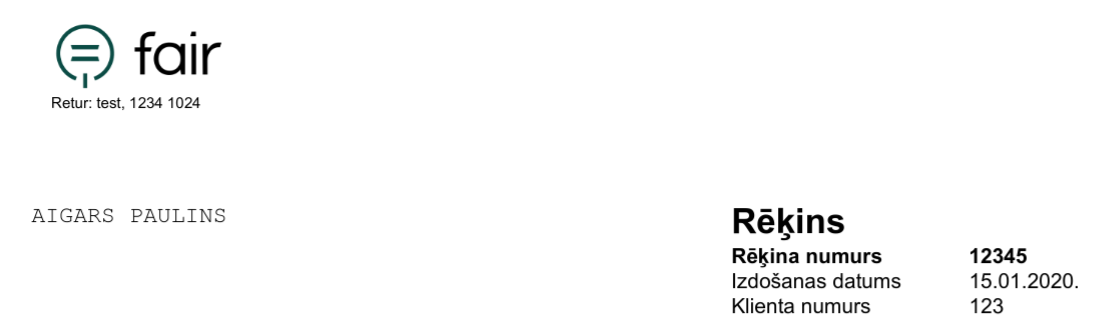
\includegraphics[scale=0.5]{stylesheet.png}}
    \caption{Izveidotā \texttt{PDF} faila galvene}
    \label{orig:pdf}
\end{figure}

%     \item izmantotās tehnoloģijas
%     \begin{itemize}
%         \item apache groovy
%         \item xml
%         \item txt
%         \item csv
%     \end{itemize}